This sections presents the \gls{DSL} Volr. \index{Volr}
The main purpose of Volr is to define clear and reproducible
experiments whose semantics are retained regardless of
the runtime environment.
It is built for the concise specification and straight-forward
translation of neural models into both artificial, as well as
spiking network models.
Volr focuses solely on the topology of networks, thus
separating the network description from generation-specific
properties of neurons or neuron populations.

The first requirement on semantic consistency explained in the previous section is met through an unambiguous
syntax, heavily inspired by lamdba calculus \cite{Pierce2002}.
Figure \ref{fig:volr-expr} shows the BNF notation for expressions, values and types
in Volr. 
Figure \ref{fig:volr-rules} lists evaluation rules for the correct
interpretation of the expressions.

% Expression figure
\begin{figure}
  \begin{tabular}[t]{l l}
    expressions 
    & \texttt{$e$ ::= $n$} \\
    & \begin{minipage}{0.6\textwidth}
      \begin{Verbatim}[mathescape,commandchars=\\\{\}]
    | \textbf{stim} $n$
    | \textbf{pop} $n\ m$
    | \textbf{tar} $n$
    | $e \otimes e$
    | \textbf{let} $x = e$ \textbf{in} $e'$
      \end{Verbatim} 
    \end{minipage} \\
    & \\ % Empty space
    values
    & \texttt{$v$ ::= $n$} \\
    & \\ % Empty space

    types
    & \texttt{$\tau$ ::= \textbf{group} $n\ m$ | \textbf{stimt} $n$ | \textbf{int} }
  \end{tabular}

  \caption{Expressions, values and types of the Volr language.}
  \label{fig:volr-expr}
\end{figure}

\begin{figure}
\begin{prooftree}
  \AxiomC{}
  \RightLabel{\hskip10pt($e1$)}
  \UnaryInfC{$\Gamma \vdash n : \mathbf{int}$}
\end{prooftree}
\begin{prooftree}
  \AxiomC{}
  \RightLabel{\hskip10pt($e2$)}
  \UnaryInfC{$\Gamma \vdash \mathbf{stim}\ n : \mathbf{net}\ 1\ n$}
\end{prooftree}
\begin{prooftree}
  \AxiomC{}
  \RightLabel{\hskip10pt($e3$)}
  \UnaryInfC{$\Gamma \vdash \mathbf{pop}\ n : \mathbf{net}\ 1\ n$}
\end{prooftree}
\begin{prooftree}
  \AxiomC{$\Gamma (x) = \tau$}
  \RightLabel{\hskip10pt($e4$)}
  \UnaryInfC{$\Gamma \vdash x : \tau$}
\end{prooftree}
\begin{prooftree}
  \AxiomC{$\Gamma \vdash e_1 : \mathbf{net}\ l\ m$}
  \AxiomC{$\Gamma \vdash e_2 : \mathbf{net}\ n\ q$}
  \AxiomC{$\Gamma \vdash w : \mathbf{float}$}
  \RightLabel{\hskip10pt($e5$)}
  \TrinaryInfC{$\Gamma \vdash \otimes\ e_1\ e_2\ w : \mathbf{net}\ l\ q$}
\end{prooftree}
\begin{prooftree}
  \AxiomC{$\Gamma \vdash e_1 : \mathbf{net}\ l\ m$}
  \AxiomC{$\Gamma \vdash e_2 : \mathbf{net}\ m\ n$}
  \AxiomC{$\Gamma \vdash w : \mathbf{float}$}
  \RightLabel{\hskip10pt($e6$)}
  \TrinaryInfC{$\Gamma \vdash \ominus\ e_1\ e_2\ w : \mathbf{net}\ l\ n$}
\end{prooftree}
\begin{prooftree}
  \AxiomC{$\Gamma \vdash e : \tau$}
  \AxiomC{$\Gamma [v : \tau] \vdash e' : \tau$}
  \RightLabel{\hskip10pt($e7$)}
  \BinaryInfC{$\Gamma \vdash \mathbf{let}\ x = e\ in\ e' : \tau$}
\end{prooftree}

  \caption{Evaluation rules in Volr.}
  \label{fig:volr-rules}
\end{figure}



The constant expression $n$ is an integer that evaluates to the type 
\texttt{\textbf{int}} ($e1$). 
Similarly to traditional functional languages, the \texttt{\textbf{let}} binding binds
the string constant $x$ to the expression $e$ when evaluating $e'$ \cite{Pierce2002}.
That constant can later be referenced in the $e'$ expression 
through the string $x$ as shown in $e2$.

The \texttt{\textbf{dense}} expression describes a fully connected
neural network layer, and is the smallest building block for networks
\gls{DSL}.
This aligns with the previous understanding of a layer, where
a \texttt{\textbf{dense}} network layer can be understood as a number of inputs,
that are densely connected to a number of outputs (see Section
\ref{sec:nn_graphs}).
To calculate the output of the layer, the layer bias is added to the
weighted input (output from the previous layer) and given 
to the activation function.
Taking into account the definition of layers as functions over vectors as described previously, each neuron 
accounts for the activation of a single dimension in the input/output vectors.
In turn, $n$ and $m$ illustrate the \textit{dimensionality} of the network,
such that the number of dimensions in the input is truncated (or expanded) to
the dimensionality of the output layer.

The $\ominus$ (parallel) operator parallelises two networks by duplicating
the input from the previous layer and merging the outputs into a single
layer ($e5$).
The input from the previous layer is replicated into both $e$ and $e'$, such
that the input dimension of the network \textit{must} be shared by the two layers ($l$).
The output from the network is stacked such that each neuron from each
population corresponds to one output neuron ($e_{out} + e'_{out}$).
This is done to preserve the meaning of each parallel population, where
a truncation would loose information.

Semantically the parallel operator provides the ability for a network to
perform specialised functions, based on the same stimulus.
In the context of neural systems such specialisations are frequently used
to balance correctness with compactness: it is cheaper in terms of neurons,
and more efficient in terms of accuracy,
to allow two subnetworks to specialise than to have one large network 
generalise \cite{Eliasmith2015}.

The $\obar$ (sequential) operator binds two networks sequentially,
such that the output layer of the first network becomes the input layer 
of the second network.
This binding is similar to the \texttt{\textbf{dense}} operation before,
in that the neurons are connected densely, but differ because the operator
can connect parallel networks.
To connect networks sequentially, it is expected that the output dimensionality of
the first network ($m$) equals that of the input of the second network, as shown in $e4$.

Taken together these constructs can express simple neural networks and
the properties of their connections. 
Figure \ref{fig:volr-examples} shows a number of example networks
that visualises four examples of networks. 


\begin{figure}
  \ContinuedFloat*
  \begin{tabular}[t]{l c}
    \begin{minipage}{0.4\textwidth}
      \begin{Verbatim}[mathescape,commandchars=\\\{\}]
\textbf{dense} 2 2
      \end{Verbatim}
    \end{minipage} & \begin{minipage}{0.4\textwidth}
      \includegraphics[width=\textwidth]{chapters/volr/example2.pdf}
    \end{minipage}

  \end{tabular}
  \caption{A network with a stimulus containing two channels.
    The stimulus is fully connected to a population with an excitatory
    weight of 1. Each circular node represents a single neuron.}
  \label{fig:volr-example1}
\end{figure}

\begin{figure}
  \ContinuedFloat
  \begin{tabular}[t]{l c}
    \begin{minipage}{0.4\textwidth}
      \begin{Verbatim}[mathescape,commandchars=\\\{\}]
\textbf{let} s$_1$ = \textbf{dense} 1 1 \textbf{in}
\textbf{let} s$_2$ = $\neg$ \textbf{dense} 1 1 \textbf{in}
(s$_1$ $\ominus$ s$_2$) $\obar$ \textbf{dense} 2 1
      \end{Verbatim}
    \end{minipage} & \begin{minipage}{0.6\textwidth}
      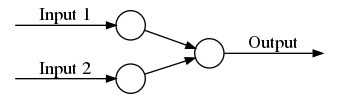
\includegraphics[width=\textwidth]{chapters/volr/example1.pdf}
    \end{minipage}
  \end{tabular}
  \caption{An illustration of a simple binary network, whose two 
	   parallel layers share the middle population of size 2.}
\end{figure}

\begin{figure}
  \ContinuedFloat
  \begin{tabular}[t]{l c}
    \begin{minipage}[b]{0.4\textwidth}
      \begin{Verbatim}[mathescape,commandchars=\\\{\}]
      \textbf{dense} 100 50
        $\obar$ \textbf{dense} 50 10
      \end{Verbatim}
    \end{minipage} & \begin{minipage}{0.5\textwidth}
      \includegraphics[width=\textwidth]{chapters/volr/example3.pdf}
    \end{minipage}
  \end{tabular}
  \caption{A larger network that can process the MNIST dataset
    as 10x10 pixel images. 
    The nodes are populations of neurons,
    where the input corresponds to the pixel size ($10\cdot10=100$) 
    and the output to the possible classes (0 - 9).
    Input and output are implicit.}
\end{figure}

\begin{figure}
  \begin{tabular}[t]{l c}
    \begin{minipage}{0.45\textwidth}
      \begin{Verbatim}[mathescape,commandchars=\\\{\}]
\textbf{let} s = \textbf{dense} 2 2 \textbf{in}
\textbf{let} l$_1$ = \textbf{dense} 2 4 \textbf{in}
\textbf{let} l$_2$ = \textbf{dense} 2 4 \textbf{in}
\textbf{let} o = \textbf{dense} 8 1 \textbf{in} 
  s $\obar$ (l$_1$ $\ominus$ l$_2$) $\obar$ o
      \end{Verbatim}
    \end{minipage} & \begin{minipage}{0.5\textwidth}
       \includegraphics[width=\textwidth]{chapters/volr/example4.pdf}
    \end{minipage}
  \end{tabular}
   \caption{An example where a two-dimensional input is split into
     two nodes and later merged into a node of a single neuron.}
  \label{fig:volr-examples}
\end{figure}


\FloatBarrier
